\chapter{Summary and Outlook}
\label{ch06}
%\mquote{The terminology is not as important as the concepts. That having been said, you might encounter different sets of terms in other places and should be able to translate between them.}{P. Clements, L. Northrop, Software Product Lines, Addison Wesley, 2002}
%\mquote{For developers writing programs for devices other than the Pocket PC, our samples should run with few if any changes.}{P. Yao, D. Durant, .NET Compact Framework Programming with C\#, Addison Wesley, 2004}
%\mquote{Your quote here.}{B. Stroustrup, The C++ Programming Language, Third Edition, Addison-Wesley, 1997}
%\mquote{It seems in the nature of individuals and organizations to attempt projects that are at the limits of their ability.\\There is no "one right way" to design and build all systems.\\..., we must plan for a series of successes.}{B. Stroustrup, The C++ Programming Language, Third Edition, Addison-Wesley, 1997}
\mquote{I would have made the book shorter, but I did not have any more time.}{E. H. Connell, Elements of Abstract and Linear Algebra, 1999}

\section{Summary}

This book has been concerned with the problem of finding better and faster ways to automate and reuse software in mobile device applications\footnote{Mobile applications, for short.}. The focus has been in (a) developing easy to implement techniques for organizing the common domain functionality in mobile product-lines that (b) enable declarative reuse of the domain functionality in mobile applications. The problem has been addressed (\fig{fig:ac-pl}): (1) by introducing attribute-based DSA supported by GAAST-enabled languages, (2) by having a structured way to interpret attributes with modularized attribute-driven transformers and finally, and (3) by using a software container abstraction to organize the domain assets of mobile application product-lines.

\begin{figure}[ht]
	\begin{center}
		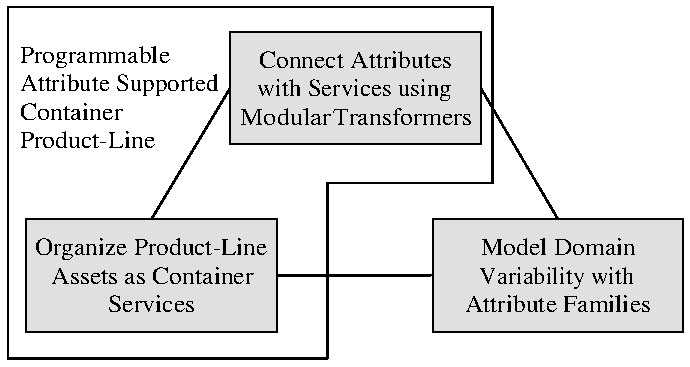
\includegraphics[width=9cm,height=!]{ch06/summary}
	\end{center}
	\caption{Attribute-Supported Container-Based Product-Lines}
	\label{fig:ac-pl}
\end{figure}

After an introduction to the main topics in \kr{ch01}, \textbf{\kr{ch02}} motivated product-lines support for the development of mobile applications and presented mechanisms for implementing mobile product-lines. \Kr{ch02} proposed to organize mobile product-lines with mobile containers, and to support such containers with DSA at the source code level.

\begin{itemize}

\item Automated product-lines are needed to support mobile applications and reuse the common functionality. The mobile product-lines factor out the common functionality of a family of applications and inject the common functionality transparently into a specific application. Automation helps to deal with the cross-cutting nature of the common functionality that is present in more than one application.

\item There are several variability mechanisms for supporting product-lines. Declarative domain-specific abstractions (DSA) supported at the programming language level help to make the domain architecture explicit and to preserve the domain model in the source code. DSA blur the distinction between a modeling phase and the coding phase, and offer support for the traceability of domain concerns in specific applications.

\item A software container serves as an architectural abstraction to organize the domain assets. Containers are known from the domain of server-side enterprise applications. When combined with attribute-based DSA \seec{ch03}, the container offers an architectural abstraction to connect the implementation of the domain assets with the declarative attribute constructs in code.

\item There are many ways to implement containers. Invasive generative containers are better suited for mobile product-lines compared to non-invasive techniques. Invasive containers supported by declarative domain-specific abstractions (DSA) offer more automation and could introduce easy domain-specific optimizations.

\item Aspect-oriented programming (AOP) engines could be used as generic invasive frameworks to implement attribute-driven transformations. Specialized transformation engines are, however, preferable for specific domains. The specifics of attribute-based DSA are utilized to create specialized attribute-driven transformers. AOP and DSA can coexists and complement each-other \see{sec.aop.dsa}. DSA support an explicit programming model and enable vertical automation. AOP-style modularization can be applied over the existing DSA language constructs. 

\end{itemize}

\noindent \textbf{\Kr{ch03}} focused on the aspects of attribute-enabled languages and the effects of \textit{attribute enabled programming} (AEP) in the software development process. GAAST was introduced as a common API of an extensible language workbench, intended to support attribute-based DSA. Several aspects of using attribute-enabled languages in the software development process were investigated.

\begin{itemize}

\item Attribute-based DSA decrease the cost of introducing custom DSA in a language, making attributes preferable for supporting iterative product-lines. Attributes expose a uniform programming model and do not require grammar modifications. Attribute-based DSA selectively customizes the semantics of existing components or language constructs.

\item Domain variability is modeled as attribute families. Each attribute family represents a domain asset of interest that needs to be automated. Inside each family, a name space organization is applied to nest attribute sub-families that define further specialization of the modeled asset. Attribute parameters model the variability ranges of individual attributes.

\item AEP is attractive for mapping MDA UML class models to source code. Unlike other approaches, e.g., marking interfaces and pseudo-syntactic marking, attribute programming fully preserves the architecture of the model in code. Attribute programming serves as an extension to the overall MDA transformation process. Attributes supported by GAAST-enabled languages move the MDA transformation concerns at the language level and offer a single transformation system to the programmers.

\item UML stereotypes and tagged values model only a subset of the AEP development scenarios. The full range of attribute-based design possibilities in UML class diagrams can be modeled in different ways. All these alternatives extend the UML class diagrams notation. None of them is better suited in all cases, reflecting the wide range of design possibilities that can be modeled by attributes.

\item Explicit attributes in the programming language level extend the semantics of the language meta-model without the need to modify or maintain its parsing tools. This results in low-cost language support for a wide range of EDSL that model the product-line abstractions.

\item Several modern general-purpose languages, e.g., NET and Java, offer support for attributes as part of their language technology. An arbitrary number of custom attributes can be introduced. Several API-s, e.g., .NET CodeDom and Reflection API-s, process the code entries annotated with attributes either before compilation or at run-time. Run-time support is enabled via the Reflection API, which uses the structural information saved in the binary meta-data.

\item The attribute processing API-s found in .NET and Java do not cover the full range of possible attribute-driven transformation scenarios. Several attribute-based transformations could be represented uniformly despite the origin of the attribute-decorated AST. Generalized and Annotated AST (GAAST) enabled languages offer uniform attribute support for processing source code, or binaries after compilation, or at run-time. When GAAST is supported as part of the language technology no third-party parsing and meta-programming tools are needed. Third-party frameworks add accidental complexity to a product-line. When GAAST is not supported in a language, several aspects of GAAST are easily emulated with any meta-programming tool, keeping the cost of introducing GAAST and attribute-based DSA at a minimum.

\item The power of GAAST languages does not stand in the expressiveness of grammars they generate, but in the transformations they apply to an existing core grammar. GAAST makes the language meta-model enhancement implicit. GAAST reduces the meta-model maintenance costs, and removes the need to rely on external third-party transformation frameworks.

\item Attributes are cheap to introduce and could be easily over-used. They should not be applied to model semantics that could be expressed in simpler ways with existing language constructs. The scope of attribute annotations needs to be carefully chosen based on the characteristics of the domain assets modeled with attributes.

\end{itemize}

\noindent \textbf{\Kr{ch04}} addressed issues related to attribute-driven variability and transformations. Modular attribute-driven transformations implement attribute-based DSA in a structured way. Transformer modularization reduces the overall cost of supporting product-lines with attributes and enables reuse of the individual transformation units.

\begin{itemize}

\item The properties of the addressed domain, attribute-based DSA for mobile product-lines, are utilized to modularize transformers. The transformation process is organized in separate transformer units based on the domain assets.

\item Inner attributes coordinate between the individual transformation units. Attribute-driven transformations treat inner attributes similarly to other explicit attributes. The similarity results in a uniform model for expressing the transformation composition semantics and enhances traceability.

\item The relations between the modeled domain assets specify the transformation workflow. Dependency lists are parsed to automatically create the transformation dependency graph. Conflicts are solved using a workflow language.

\item The properties of the specific language meta-model are utilized to vertically modularize attribute-driven transformers. The transformation strategy is structured according to the structural nesting in the meta-model hierarchy. Attribute semantics are separated between the layers. Layering is enforced with special syntax. The operations in each layer are made declarative with specialized strategy operations.

\item Meta-attributes express transformation cross-cutting concerns (CCCs) declaratively in a GAAST-enabled language. Meta-attributes are processed separately outside the individual transformers with generic tools. When an attribute is defined, its definition is decorated with meta-attributes representing the generic concerns that need to be validated for that specific attribute.

\item Attribute dependencies are an important attribute transformation concern that is expressed declaratively using meta-attributes. Attribute dependencies enable expressing the valid attribute usage context with regard to other attributes in a way similar to representing grammar parser rules. The semantics of the dependency attribute are checked with specialized tools.

\end{itemize}

\noindent \textbf{\Kr{ch05}} summarized and evaluated the concepts presented in this book by presenting MobCon, a generative mobile container framework specialized for addressing J2ME MIDP non-functional application concerns.

\begin{itemize}

\item J2ME MIDP applications form a domain of interest that exhibits redundant behavior in the form of cross-cutting non-functional concerns. An extended product-line for supporting MIDP domain assets, based on the technology presented in this book, was created. MobCon was used to study the effects of attribute-based DSA and attribute-drive transformations, serving as a basis for the generalization of the concepts presented in the previous chapters.

\item A GAAST-like representation was implemented for the Java dialect supported by the MIDP. It was combined with a customizable transformation framework to manage the workflow of the transformation process. Transformation units are modeled as different plug-ins based on the attribute families that cover the addressed MIDP concerns.

\item The container abstraction constitutes a centralized point to support variability in a mobile software product-line. Mobile containers are a specialization of the container architectural abstraction for supporting automated mobile product-lines. Mobile containers deal with client-side automation issues. Their functionality and service support extends from the mobile device to the server-side. The container impersonates the mobile client to the rest of the environment services. 

\item Several MIDP concerns, e.g., data persistence, screen management, image adaptation, data encryption and networking, are organized as part of a mobile container. The container is modeled as a set of MobCon plug-ins specialized for MIDP. Each plug-in transforms an attribute family, and generates also container infrastructure code to be placed on the server-side as needed.

\item The MobCon framework is designed to be extensible. New plug-ins can be added to support new MIDP concerns or existing plug-ins can be modified. New domains could also be supported by a new set of plug-ins. MobCon uses the plug-in meta-data to calculate the transformation workflow, and enables the developers to customize the workflow for specific applications.

\end{itemize}

%It seems in the nature of individuals and organizations to attempt projects that are at the limits of their ability.\\
\mquote{There is no "one right way" to design and build all systems. ..., we must plan for a series of successes.}{B. Stroustrup, The C++ Programming Language, Third Edition, Addison-Wesley, 1997}

\cendsection{Limitations and Outlook}

%\mquote{It seems (to be) in the nature of individuals and organizations to attempt projects that are at the limits of their ability.\\There is no "one right way" to design and build all systems. ..., we must plan for a series of successes.}{B. Stroustrup, The C++ Programming Language, Third Edition, Addison-Wesley, 1997}

\noindent As discussed in \kr{ch03}, attribute-based DSA model only a limited subset of EDSL. Attri\-bu\-tes by definition decorate existing entities. They cannot implement arbitrary EDSL or DSL constructs. Attributes are used in this book to declaratively modify the semantic of OO components. Only static decorations of structural elements are utilized to implement the MobCon container framework.

Attribute transformations addressed in this book \seec{ch04} are specialized to support OO mobile device software product-lines. The modularization is dependent on the domain assets and on the orthogonality of the assets. Only the transformations applied over the structural decoration of OO components with attributes are explored. The functionality of the methods is presented internally as a series of code blocks. A finer grained representation may be needed for other domains.

The solution for supporting mobile software product-lines was investigated in details. The introduced concepts were evaluated by various prototypes. There are also several open areas for further exploration.

\begin{itemize}

\item \textbf{Further improvement of different aspects of the introduced technologies.} One area for future work would be to investigate of the impact of the GAAST-like organization API for representing the annotated source, binary, and run-time in the context of a specific compiler. That is, to find out the best organization for a compiler with integrated GAAST support. Such a compiler needs to have an API-like front-end accessible from the programming language level. It can then be used to support transparently GAAST-based transformations. Only the static aspects of GAAST-based transformations were explored in this book. Depending on level of reflection supported in the language, GAAST could serve also as an advanced reflective meta-programming system for supporting dynamic attribute-driven transformations.

Another area for future work is to add more MIDP services to MobCon to support other MIDP related tasks. More variability could also be supported for the existing MIDP domain assets. Given the extensibility of MobCon, new features can be added to the current set of MIDP plug-ins to extend the MIDP support. The combination of attribute-based DSA with wizards and visual models could also be explored.

It is also possible to combine the features of Tango and MTE prototypes into a single attribute-driven transformation engine. The specific transformation issues were properly investigated in Tango and MTE. A combined transformation engine could also support a bigger number of specialized transformer operations. It could also enable the developers to distinguish between changing a class in place and creating an adapter or decorator \cite{dpatterns} for a class. The declarative common operations, e.g., declaration and enforcement of attribute dependencies, part of the ADC prototype \seec{ch04}, could also be generalized and made part of the special operations supported by a unified framework. An extensible plug-in architecture to support meta-attributes could be created.

\item \textbf{Areas for future research.} An interesting topic for future research is to investigate the applicability of the technology developed in this book to another domain, for example, to automate web service programming concerns. Some of the examples given in the thesis to illustrate various aspects of GAAST-enabled languages and attribute dependencies were motivated from the domain of web services. 
In the large, it would be also very interesting to evaluate what kind of domains and what types of product-lines could better benefit from attribute-based DSA supported containers.

\end{itemize}




 